\section{Software Design}
\phantomsection
\subsection{UML Modeling}
In the current chapter is represented and described the architecture of OpenMedia application. It contains a set of relevant diagrams modeled in UML language. The diagrams provide a fundamental documentation an description of the system structure and behavior.

The first thing which should be defined is how user will interact with the application. Therefore a use case diagram was modeled to show the set of actions offered at user's disposal. The client part of the application represents a browser web page. There are five main actions which the application user can performed. The operations can be seen in figure \ref{use_case}. When the applications is opened, the user can perform the basic word frequency search. The second actions that asks the application to perform an analysis is the trend detection. Here the user will be able to set the intervals on which the trends disclosure is achieved. The remaining options of interaction with the applications aims to visualize the information on the performed tasks. For instance the action of displaying the word frequency renders the density of a specific word, under the form of a plot chart. Trend detection result has an analogical approach of representation.

\begin{figure}[!ht]
\centering
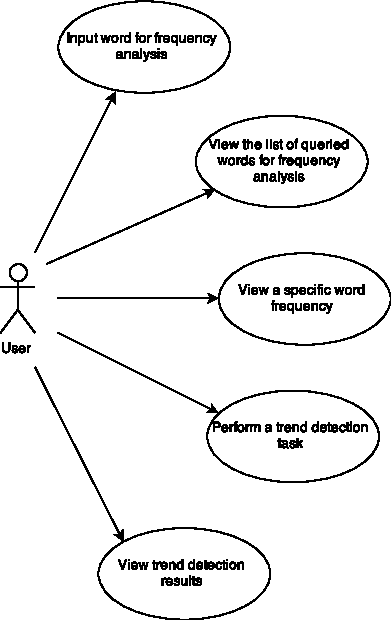
\includegraphics[width=8cm]{2_use_case}
\caption{User Use Case Diagram}\label{use_case}
\end{figure}

To offer a detailed overview of how the entire system works, a set of sequence diagrams are provided. They show key parts of the platform and the way they interact. Moreover it is crucial to depict the depth of chain of events happening in the background.
For instance the sequence diagram, shown in figure \ref{user_sequence}, specifies what happens when a user does a simple word frequency query. First of all the user does an HTTP request over the browser in order to get the application page. Now he is able to interact with OpenMedia. When he requests a word frequency, two things are performed. First is an AJAX request that aims to launch the task. The second thing is subscribing to a websocket channel that allows to receive the task finished notification. The web application fires an asynchronous job on the Sidekiq server. When the job has finished, it sends an HTTP request to the websocket server. The next and the last thing is that client's web page receives the notification because it was subscribed to the channel.

\begin{figure}[!ht]
\centering
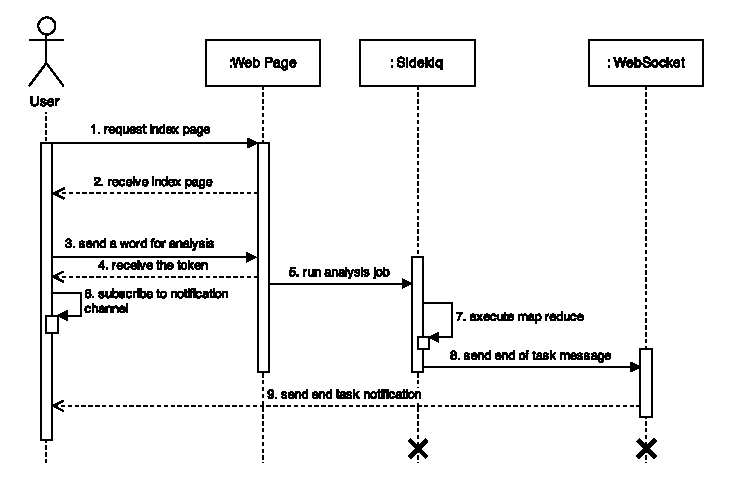
\includegraphics[width=18cm]{2_user_sequence}
\caption{User Sequence Diagram}\label{user_sequence}
\end{figure}

The client part is only one part of the application. The data gathering side consists of three main steps. Each one is described in the sequence diagrams illustrated below. Their behavior looks similar, nevertheless each has unique characteristics worth pointing out.

First step of data gathering process is fetching the articles, which is depicted in figure \ref{fetcher_sequence}. The entry point of the application is a makefile which runs ruby scripts. Every media source has a custom fetcher class, nevertheless they all posses the same interface. The main script instantiates every type of fetcher and runs it. The articles retrieving class is smart enough to be able get the all the accessible articles in an iterative way, followed by saving the data on the files storage. The entire process is straight and monotonous. The only external dependency here is for public media providers server to be up and running.

\begin{figure}[!ht]
\centering
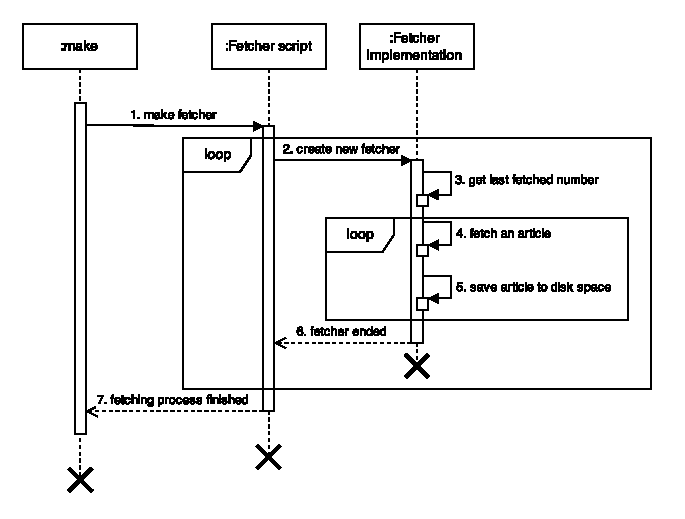
\includegraphics[width=18cm]{2_fetcher_sequence}
\caption{Article fetcher sequence diagram}\label{fetcher_sequence}
\end{figure}

The sequence diagram, figure \ref{parser_sequence}, represents the action of parsing the fetched articles. It is the second step in the data gathering cycle. It works analogically as the first part. Due to the fact that every media source has their own way to represent the article concludes that each source should have a custom parser. But again with a similar interface. The parsing script instantiates a custom parser object and runs it. The custom object is able to retrieve the fetched articles from the file storage, extract the meaningful information and save it back to a database. This action is represented on the diagram in a iterative way.

\begin{figure}[!ht]
\centering
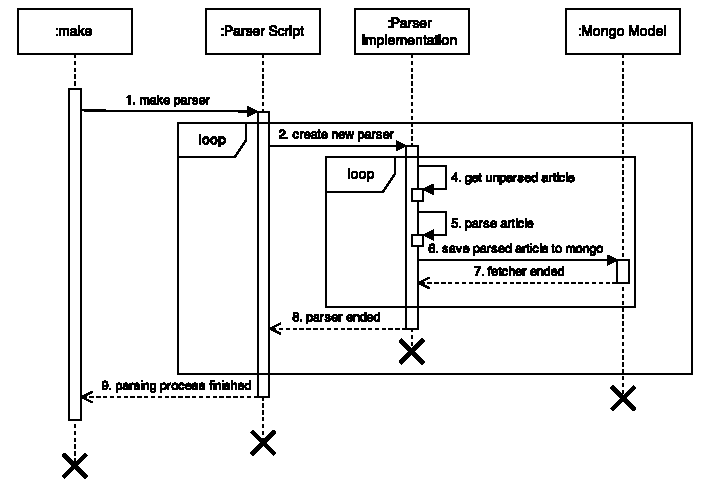
\includegraphics[width=18cm]{2_parser_sequence}
\caption{Article parser sequence diagram}\label{parser_sequence}
\end{figure}

The last, time consuming, step in the data mining cycle is executing natural language processing on the given data. This part is decisive in the OpenMedia project. Running analysis on simple chunks of text is inefficient. Which is why text should be annotated with metadata such as part of speech, lemmatized forms etc. The way it differs from the previous steps is that it does not need customized classes. Presumably the articles are already saved under the same form, the scripts iteratively extracts articles. Each iteration undergoes a sequence of NLP operations, which can be observed in the diagram figure \ref{nlp_sequence}. The operations are: tokenization, part of speech tagging, and lemmatization. The last step of an iteration is splitting the articles and saving back to database under a different form.

\begin{figure}[!ht]
\centering
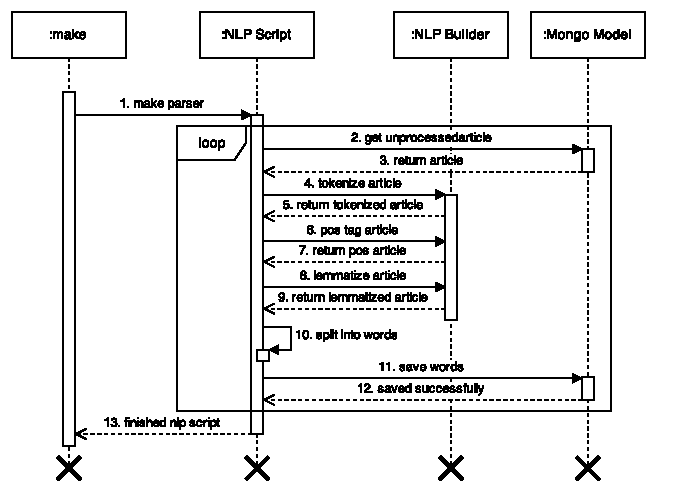
\includegraphics[width=18cm]{2_nlp_sequence}
\caption{NLP script sequence diagram}\label{nlp_sequence}
\end{figure}

Until now every step of data mining process was described particularly. The activity diagram, drawn below figure \ref{data_mining_activity}, represents, on an abstract level, the sequence of actions performed on the data gathering part of the application. Every executed step depends on the previous one. There is also the final part, that was not mentioned in the sequence diagrams. This part performs a series of tasks which preprocess the tokenized data. The resulted data is optimized for frequency analysis tasks. More details will be provided in the implementation chapter of the report.

\begin{figure}[!ht]
\centering
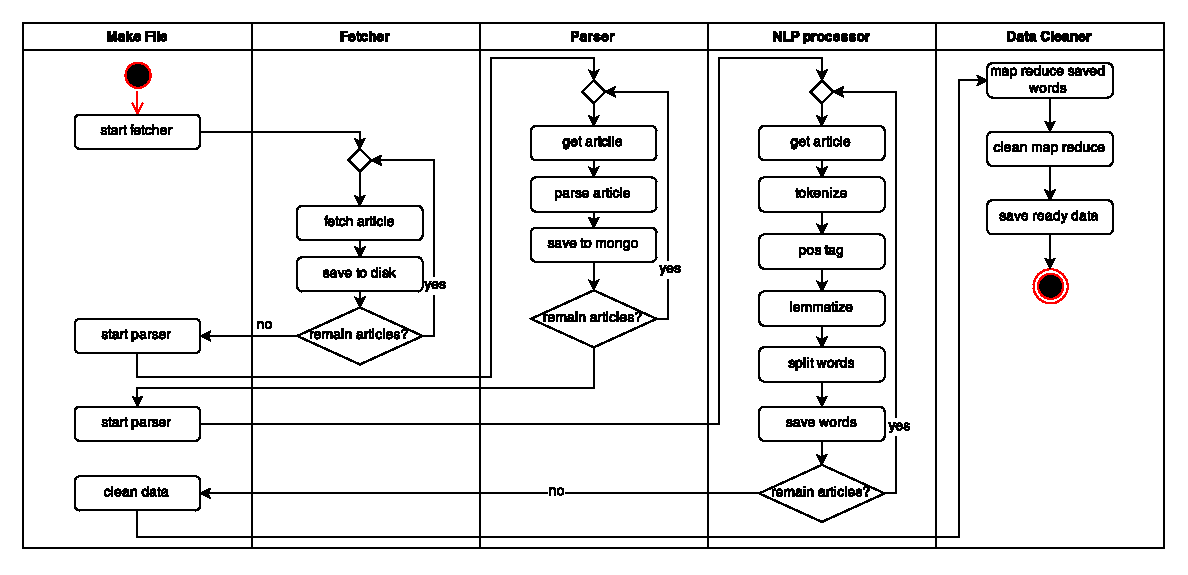
\includegraphics[width=18cm]{2_data_mining_activity}
\caption{Data Mining Activity Diagram}\label{data_mining_activity}
\end{figure}

Going back to the client part of the application, in the figure \ref{app_state_diagram} is represented a state diagram. Due to the fact that the amount of operations are limited offered by OpenMedia, denotes that there is a narrow amount of states that an application user can be in. All the application states are mapped to a browser page. First step is the index page of OpenMedia. Here user is able to input words for frequency analysis. On top of the page a panel is render that can get into almost every state. Another detail is that the client part of the software is build on RESTfull concept, which means that every state of the application can be accessed via an URI. Another application state is the trend detection page. Here user is able to perform trend disclosure operations by specifying the intervals of time. The remaining states are related only to visualizing the information. There are two states for browsing the performed queries and other two for data visualization.

\begin{figure}[!ht]
\centering
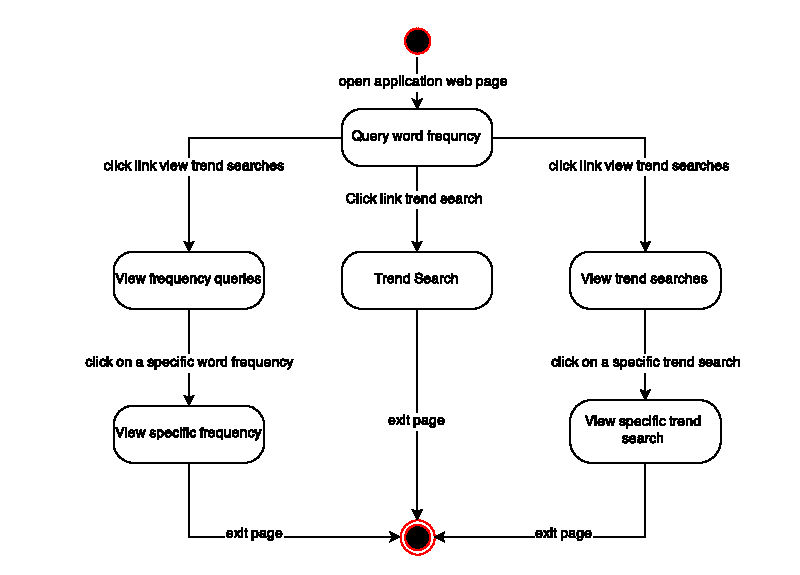
\includegraphics[width=15cm]{2_app_state_diagram}
\caption{Application State Diagram}\label{app_state_diagram}
\end{figure}

In the following part of this chapter is described the most important class diagrams of OpenMedia. Most of them are related to the data mining part of the application. Information about the system components interaction is not enough for understanding the platform. The class diagrams can deliver information under a higher level of granularity, hence the system becomes more easy to comprehend.

Each step of the data gathering aspect of OpenMedia has class diagram. It was mentioned that every custom fetcher should have it's own implementation but with a similar interface. This statement is emphasised in figure \ref{fetcher_class}. Fetcher is the abstract class. It has a set of messages which are implemented by the custom implementations, such as UnimediaFetcher, TimpulFetcher and PublikaFetcher. Fetcher class aggregates SmartFetcher class. SmartFetcher encapsulates the logic of requesting a web page where the article is represented.

\begin{figure}[!ht]
\centering
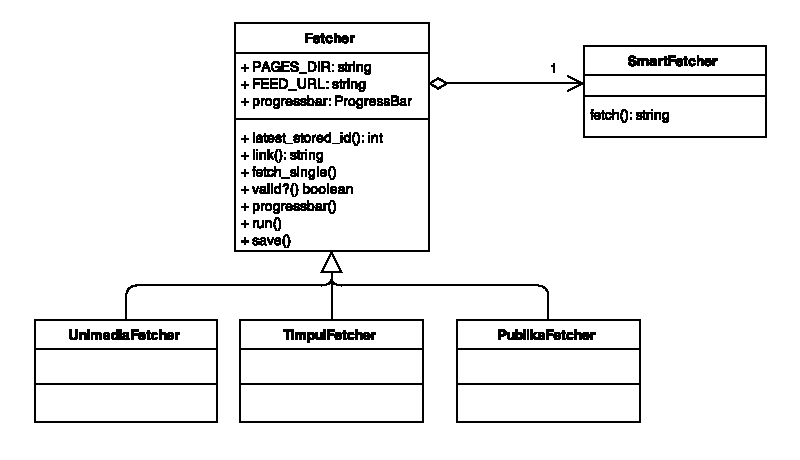
\includegraphics[width=16cm]{2_fetcher_class}
\caption{Fetching Class Diagram}\label{fetcher_class}
\end{figure}

Next class diagram is depicting the parsing objects. The conceptual model is done in an analogical way. An abstract class is predefine and has a set of predefined messages. The methods denotes the possible actions needed to successfully get an article from file storage, parse it and save it to a database. The implementations of the abstract class are UnimediaParser and TimpulParser. The Parser class has an association with ParsedPage class. ParsedPage is a MongoDB model and it is used to interact with the database in language friendly way. The rest of database models are be described below.

\begin{figure}[!ht]
\centering
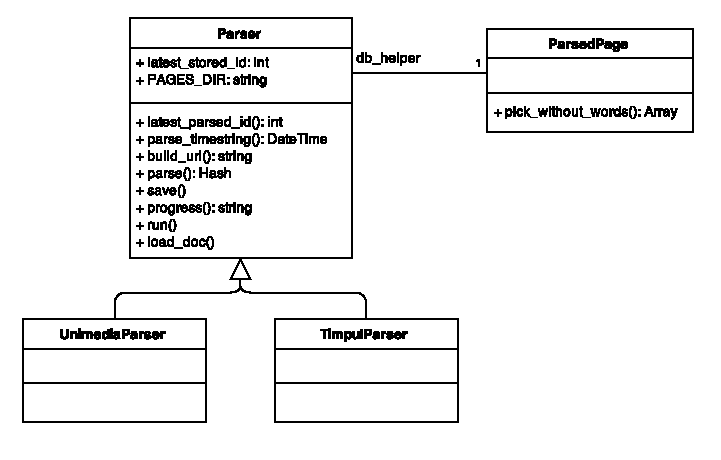
\includegraphics[width=16cm]{2_parser_class}
\caption{Parsing Class Diagrams}\label{parser_class}
\end{figure}

The last step of the data gathering platform is the natural language processing part. The class structure is much simpler. BatchRacaiFetcher class has association relationships with ParsedPage and Word model classes. Both are used for extracting data and saving it back. The main class aggregates RacaiBuilder. RacaiBuilder class is used for applying NLP actions on a given input. It is constructed under a builder pattern. This offers to developers a high flexibility, the NLP actions can be performed in any sequence. The private methods encapsulate the communication via SOAP service. Under the hood the NLP actions actually are request made to a web server. The details of this part is provided in chapter three of the report.

\begin{figure}[!ht]
\centering
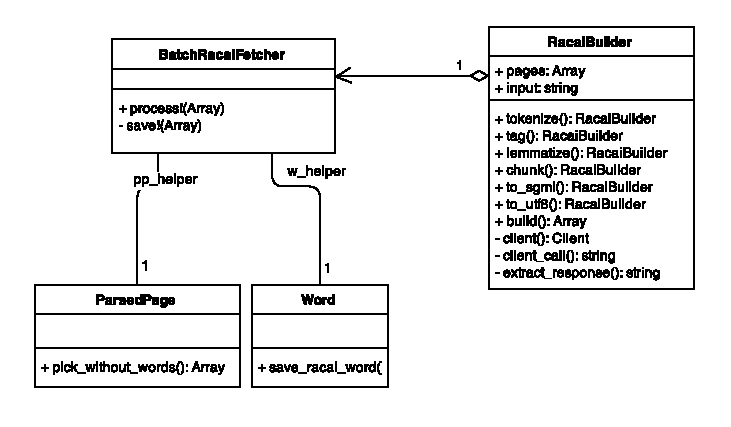
\includegraphics[width=16cm]{2_nlp_class}
\caption{NLP Class Diagram}\label{nlp_class}
\end{figure}

Mongo models provide means to interact with the database. OpenMedia platform uses MongoDB as the primary database. The fields illustrated in the class diagram, figure \ref{model_class}, are mapped to the fields in database. All models inherit from Mongoid::Document class. Mongoid is the ORM used to create models in ruby. The inheritance marks the child class that it is used for database interactions. It also offers a set of messages that allows database operations. Such as finding an element, saving an element, different other type of queries.

\begin{figure}[!ht]
\centering
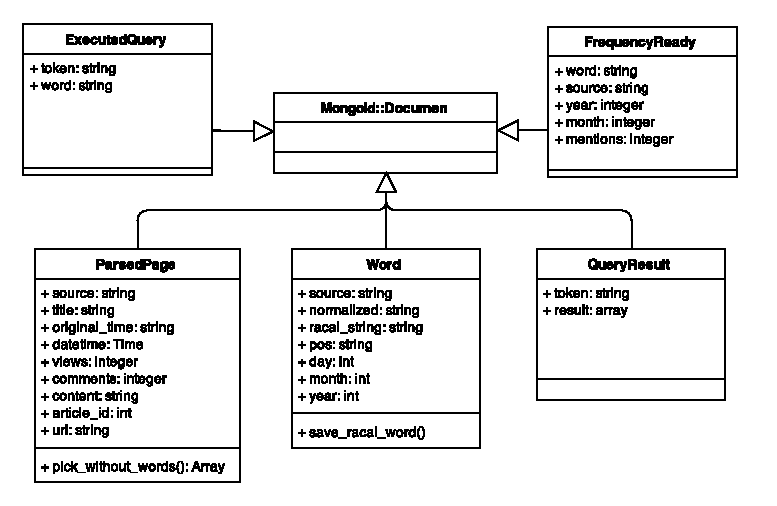
\includegraphics[width=16cm]{2_model_class}
\caption{Mongo Models Class Diagram}\label{model_class}
\end{figure}

The platform modules and their behavior were described until now. Another important part of the application is the set of libraries it uses and their purpose, depicted in figure \ref{component_diagram}. Because the project is divided in two parts there are two set of dependencies and libraries. The data mining part is a console applications, hence the set of required libraries is small. The essential library is rest\_client, used for requesting web pages and getting their content. Nokogiri is used for parsing HTML and extracting the necessary elements. Savon is a library for SOAP communications, needed for NLP processing. Mongoid is used for database communication, as it was discussed above. The enumerated libraries sums up the set of requirements needed for data gathering.

The client part of application requires more libraries because it consists from more logical components. Some gems (a ruby term for library) are shared between the logical components, for example Mongoid. Sinatra framework is used to build the web applications. The main goal is to handle client's HTTP requests. Faye library is used to host the websocket server. It is handy because it provides a higher level of functionality than a simple websocket. Haml gem aims to process the haml files for creating web page content. Haml is a dialect of HTML, simply put another markup language. Sidekiq is a library used for running asynchronous jobs. Redis is a dependency required by Sidekiq and it is used as a message queue system. D3 is a JavaScript library used for drawing plots and charts. This sums it up. Of cores there are also other dependency libraries. The good thing about developing ruby applications is that gems and their dependencies are usually managed by bundler, a handy tool dedicated to solve the dependency problem.
\begin{figure}[!ht]
\centering
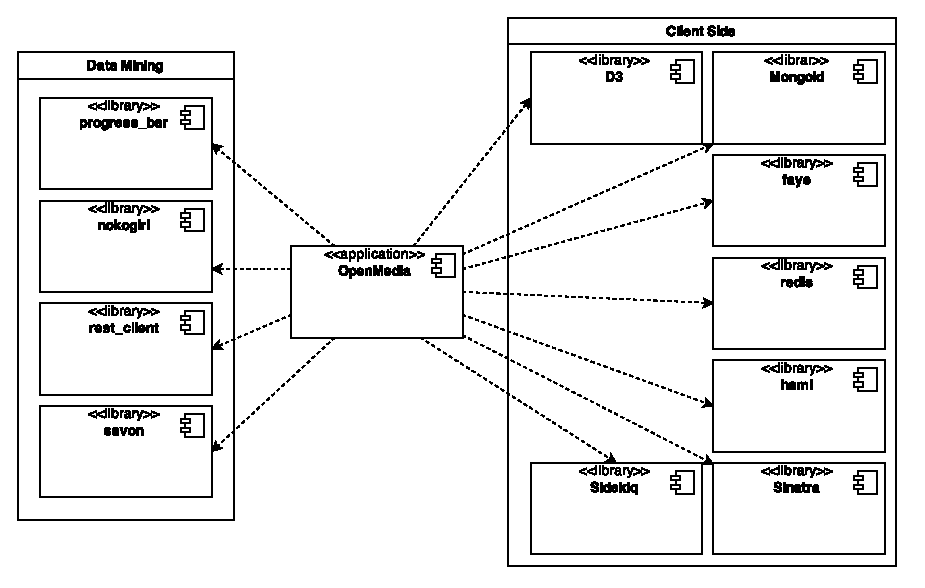
\includegraphics[width=16cm]{2_component_diagram}
\caption{Component Diagram of OpenMedia}\label{component_diagram}
\end{figure}

The deployment diagram gives a good understanding of the whole system. OpenMedia platform has a complex structure and consist of more than a few modules, it is represented in figure \ref{deployment}. In order to run the application not every module is needs to run. Data mining application is a console ruby applications which only requires to run once in a while in order to keep the database with up to date content. Moreover the NLP server is an external web service maintained by \emph{Institutul de Cercetare pentru Inteligență artificială Mihai Drăgănescu, Academia Română}. The rest of platform modules were mentioned here and there in the report. The diagram is useful because it provides a big picture of system.

\begin{figure}[!ht]
\centering
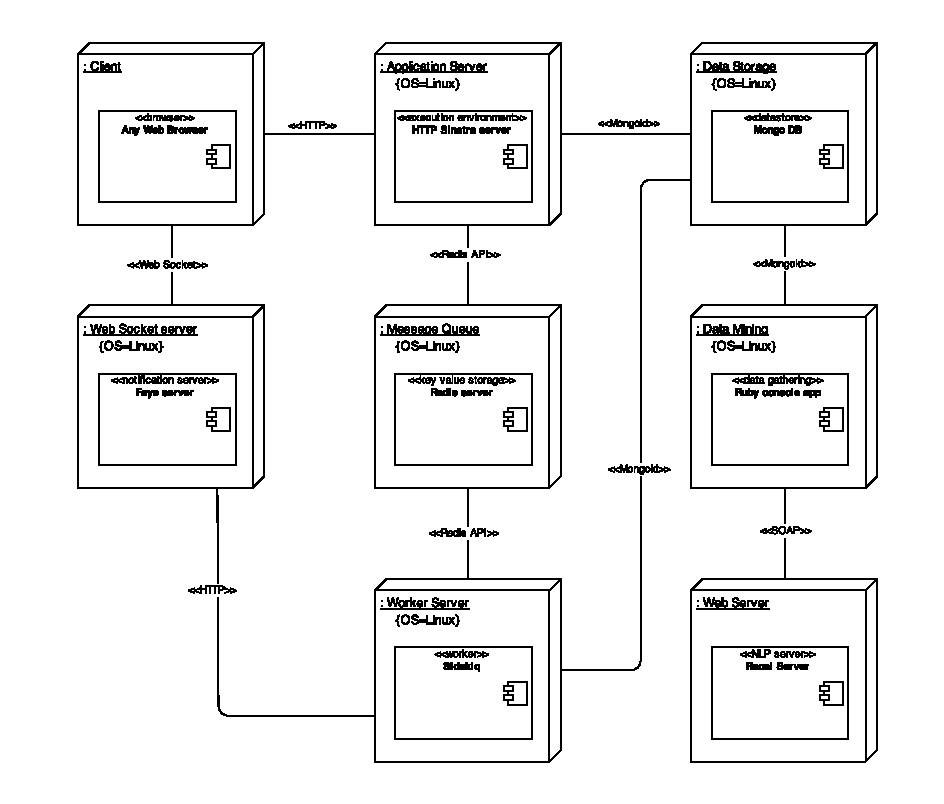
\includegraphics[width=18cm]{2_deployment}
\caption{Deployment Diagram}\label{demployment}
\end{figure}
\clearpage

Therefore the UML diagrams concentrate on the application prototype. They cover the most useful standard diagrams: use case diagrams, sequence diagrams, class diagrams, state diagrams, activity diagrams, components diagrams and deployment diagrams. All diagrams express the relationships, structural and behavioral aspects of the system.

The implementation chapter focuses on the provided UML design, implements the classes and follows the use cases and sequence diagrams to define the flow of the application. The application components and dependencies will probably extend to a bigger degree.

This concludes the UML description of the project, that aimed at presenting the most relevant aspect of the system and covering the general architecture of the application. The UML methodology offered a good documentation basis and a clear view on requirements of the software.